\begin{figure}[h]
\centering
    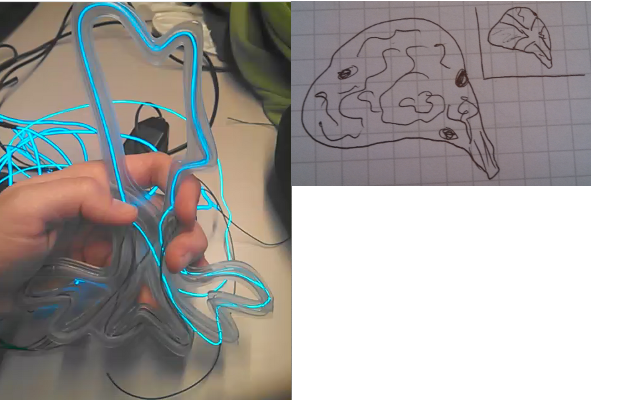
\includegraphics[width=3.4in]{figures/placeholder/teaser.png}
\caption{A novel neon sign (a) and a touch-sensitive brain (b) designed with our pipe tool and fabricated on a consumer-grade 3D printer.  (c) and (d) show the structure of the internal pipes generated by our tool.  \bjoern{will this be the robot or the UIST sign?}}
\label{fig:teaser}
\end{figure}

\section{Introduction}

\tovi{condense}
Makers, as well as professional designers, leverage 3D printers as tools for design work.  A wide array of objects, ranging from bicycle helmets to jewelry to video game controllers, are now prototyped or even manufactured using these machines.  However, most devices fabricated by 3D printers are passive.  We propose a novel technique involving the removal of material from the interior of 3D models, prior to printing, to create pipes and other cavities.  These pipes can be filled, post-print, by a variety of media that enable input, display, and tactile feedback.  This {\em subtractive} approach is complementary to {\em additive} approaches that try to print different materials, such as conductors. While our approach requires manual assembly afterwards, it opens up a large useful design space on commonly available 3D printers, allowing makers to create objects like those in Figure \ref{fig:teaser}.

These channels introduce an entire design space of opportunities for adding interactivity to these objects. For example, copper material can fill the channels, to allow for standard electronic components to be easily integrated after the printout; air can be pumped through to create tactile output; or electroluminescent wire can be threaded through to create computer-controlled visual output.

\tovi{Im not sure this emphasis on
redirection/centralization is
that important (probably
does require this entire
paragraph)}
\bjoern{Maybe focus on this on expanding the utile and applicability of sensing techniques recently introduced in hci into types of objects not initially intended for.}
The use of pipes can allow for \emph{redirection} and \emph{centralization} of active components to various locations on a printed object's surface.   For example, to create a touch-sensitive toy as in Figure \ref{fig:teaser}, a maker can select several locations of interest on the brain.  After creating pipes to those locations and printing her object, she can fill the pipes with conductive paint.  For sensing, she need only connect a single wire to a shared out of all the tubes, and can distinguish them via Swept Frequency Capacitve Sensing \cite{Sato-touche}.  In this way, she has only a single active element (the microcontroller setup), but her otherwise-inert 3D printed object (the brain) has several active sensing locations.

Pipes can also be used for sending media on a specified route through an object; for example, neon signs are created by evacuated glass tubes formed into a specific path.  Electricity is run through the near-vacuum, and this makes the path visible.  If our maker wants to build such a sign, she can substitute Electroluminescent (EL) wire for the evacuated glass and electricity: she need only design a path for the wire to be fed through and then create pipes along that path.

The generation of these pipes, however, is not trivial.  Pipes need to have maximum possible bend radius to ease the insertion of media post-print.  Independent pipes should not intersect, as this could lead to electrical shorting or other problems.  Pipes should not pass too close to the surface (unless they are being used for display purposes).  Consumer-grade 3D printers do not guarantee air- or water-tightness of their prints, so more than one layer may be required to prevent fluid leakage.  Pipes for applications like neon signs must have an Euler tour through them: this allows a single EL wire to pass through every edge on the pipe graph.  No tools yet exist for this design task.  We have developed techniques for minimizing the bending energy of, enforcing non-intersection with, and avoiding the surface for pipes, as well as expanding user-specified paths and generating Euler tours.  These techniques are embodied in our software tool to enable makers to create pipe-powered interfaces.

\bjoern{A bit repetitive with col 2 of page 1. There's opportunity for consolidation and shortening.}
Many existing sensing and actuation approaches, such as FlyEye \cite{Wimmer-flyeye}, Jamming User Interfaces \cite{Follmer-jamming}, and Touch\'{e} \cite{Sato-touche}, can be enhanced by the use of pipes.  Pipes allow makers utilizing these sensing and actuation strategies to locate input and output at arbitrary points on an object's surface.  Thus, we leverage these existing techniques for sensing and actuation while our work's novelty is in \emph{internal modeling} for 3D printing and the \emph{redirection} of IO to arbitrary locations on a device.

Our work makes the following contributions to the field of digitally fabricated interactive objects:

\begin{itemize}
\item We lay out a design space of pipes and their openings, contained media, topologies, and design focus.
\item We offer algorithms and techniques for routing pipes, as well as a design tool implementing them.
\item We showcase a set of examples, enabled by our modeling tool and exploring new points in the design space.
\item We describe the interaction possibilities of pipes, including prior work as well as uncharted possibilities. \bjoern{This last point sounds a t like the first.}
\end{itemize}